
\documentclass[a4paper,14pt]{extreport}
\usepackage{cmap} % Улучшенный поиск русских слов в полученном pdf-файле
\usepackage[T2A]{fontenc} % Поддержка русских букв
\usepackage[utf8]{inputenc} % Кодировка utf8
\usepackage[english,russian]{babel} % Языки: русский, английский
%\usepackage{pscyr} % Нормальные шрифты
\usepackage{amsmath}
\usepackage{geometry}
\geometry{left=30mm}
\geometry{right=15mm}
\geometry{top=20mm}
\geometry{bottom=20mm}
\usepackage{titlesec}
%\usepackage[ruled,longend]{algorithm2e}
\usepackage{textgreek}
\usepackage{algpseudocode}
\usepackage{pgfplots}
\pgfplotsset{compat=1.9}
\usepackage{algorithm}
\renewcommand{\listalgorithmname}{Список алгоритмов}
\floatname{algorithm}{Алгоритм}
\usepackage{amssymb}
\titleformat{\section}
{\normalsize\bfseries}
{\thesection}
{1em}{}
\titlespacing*{\chapter}{0pt}{-30pt}{8pt}
\titlespacing*{\section}{\parindent}{*4}{*4}
\titlespacing*{\subsection}{\parindent}{*4}{*4}
\usepackage{setspace}
\usepackage{mathtools}
\usepackage{float}
\DeclarePairedDelimiter\bra{\langle}{\rvert}
\DeclarePairedDelimiter\ket{\lvert}{\rangle}
\DeclarePairedDelimiterX\braket[2]{\langle}{\rangle}{#1 \delimsize\vert #2}
\onehalfspacing % Полуторный интервал
\frenchspacing
\usepackage{indentfirst} % Красная строка
\usepackage{titlesec}
\titleformat{\chapter}{\LARGE\bfseries}{\thechapter}{20pt}{\LARGE\bfseries}
\titleformat{\section}{\Large\bfseries}{\thesection}{20pt}{\Large\bfseries}
\usepackage{listings}
\usepackage{xcolor}


\usepackage{pgfplots}
\usetikzlibrary{datavisualization}
\usetikzlibrary{datavisualization.formats.functions}
\usepackage{graphicx}
\newcommand{\img}[3] {
	\begin{figure}[h]
		\center{\includegraphics[height=#1]{assets/img/#2}}
		\caption{#3}
		\label{img:#2}
	\end{figure}
}
\newcommand{\boximg}[3] {
	\begin{figure}[h]
		\center{\fbox{\includegraphics[height=#1]{assets/img/#2}}}
		\caption{#3}
		\label{img:#2}
	\end{figure}
}
\usepackage[justification=centering]{caption} % Настройка подписей float объектов
\usepackage[unicode,pdftex]{hyperref} % Ссылки в pdf
\hypersetup{hidelinks}
\newcommand{\code}[1]{\texttt{#1}}
\usepackage{icomma} % Интеллектуальные запятые для десятичных чисел
\usepackage{csvsimple}

\usepackage{color} %use color
\definecolor{mygreen}{rgb}{0,0.6,0}
\definecolor{mygray}{rgb}{0.5,0.5,0.5}
\definecolor{mymauve}{rgb}{0.58,0,0.82}



\definecolor{darkgray}{rgb}{.4,.4,.4}
\definecolor{purple}{rgb}{0.65, 0.12, 0.82}

% Для листинга кода:
\lstset{ %
	language=c,                 % выбор языка для подсветки (здесь это С)
	basicstyle=\small\sffamily, % размер и начертание шрифта для подсветки кода
	numbers=left,               % где поставить нумерацию строк (слева\справа)
	numberstyle=\tiny,           % размер шрифта для номеров строк
	stepnumber=1,                   % размер шага между двумя номерами строк
	numbersep=5pt,                % как далеко отстоят номера строк от подсвечиваемого кода
	showspaces=false,            % показывать или нет пробелы специальными отступами
	showstringspaces=false,      % показывать или нет пробелы в строках
	showtabs=false,             % показывать или нет табуляцию в строках
	frame=single,              % рисовать рамку вокруг кода
	tabsize=2,                 % размер табуляции по умолчанию равен 2 пробелам
	captionpos=t,              % позиция заголовка вверху [t] или внизу [b] 
	breaklines=true,           % автоматически переносить строки (да\нет)
	breakatwhitespace=false, % переносить строки только если есть пробел
	escapeinside={\#*}{*)}   % если нужно добавить комментарии в коде
}


\begin{document}
	%\def\chaptername{} % убирает "Глава"
	\thispagestyle{empty}
	\begin{titlepage}
		\noindent \begin{minipage}{0.15\textwidth}
			
\includegraphics[width=\linewidth]{img/b_logo}
		\end{minipage}
		\noindent\begin{minipage}{0.9\textwidth}\centering
			\textbf{Министерство науки и высшего образования Российской Федерации}\\
			\textbf{Федеральное государственное бюджетное образовательное учреждение высшего образования}\\
			\textbf{~~~«Московский государственный технический университет имени Н.Э.~Баумана}\\
			\textbf{(национальный исследовательский университет)»}\\
			\textbf{(МГТУ им. Н.Э.~Баумана)}
		\end{minipage}
		
		\noindent\rule{18cm}{3pt}
		\newline\newline
		\noindent ФАКУЛЬТЕТ $\underline{\text{«Информатика и системы управления»}}$ \newline\newline
		\noindent КАФЕДРА $\underline{\text{«Программное обеспечение ЭВМ и информационные технологии»}}$\newline\newline
		
		\begin{center}
			\noindent\begin{minipage}{1.1\textwidth}\centering
				\Large\textbf{  Отчет по лабораторной работе №6}\newline
				\textbf{по дисциплине <<Операционные системы>>}\newline
			\end{minipage}
		\end{center}
		
		\noindent\textbf{Тема} $\underline{\text{Системный вызов open()~~~~~}}$\newline\newline
		\noindent\textbf{Студент} $\underline{\text{Зайцева А. А.~~~~~~~~~~~~~}}$\newline\newline
		\noindent\textbf{Группа} $\underline{\text{ИУ7-62Б~~~~~~~~~~~~~~~~~~~~~}}$\newline\newline
		\noindent\textbf{Оценка (баллы)} $\underline{\text{~~~~~~~~~~~~~~~~~~~~}}$\newline\newline
		\noindent\textbf{Преподаватель} $\underline{\text{Рязанова Н. Ю.}}$\newline\newline\newline
		
		\begin{center}
			\vfill
			Москва~---~\the\year
			~г.
		\end{center}
	\end{titlepage}


\chapter{Системный вызов open()}

Системный вызов open() открывает файл, указанный в pathname. Если указанный файл не существует, он может (необязательно) (если указан флаг O\_CREAT) быть создан open().

\begin{lstlisting}[language=c, caption=Системный вызов open()]
#include <sys/types.h>
#include <sys/stat.h>
#include <fcntl.h>

int open(const char *pathname, int flags);
int open(const char *pathname, int flags, mode_t mode);
\end{lstlisting}

Возвращаемое значение open() - это дескриптор файла, небольшое неотрицательное целое число, которое используется в последующих системных вызовах для ссылки на открытый файл.

Первый аргумент - имя файла в файловой системе: полный путь к файлу или сокращенное имя.

Второй аргумент - это режим открытия файла, представляющий собой один или несколько флагов открытия, объединенных оператором побитового ИЛИ. Список доступных флагов: \\


\texttt{O\_EXEC} --- открыть только для выполнения (результат не определен, при открытии директории).

\texttt{O\_RDONLY} --- открыть только на чтение.

\texttt{O\_RDWR} --- открыть на чтение и запись.

\texttt{O\_SEARCH} --- открыть директорию только для поиска (результат не определен, при использовании с файлами, не являющимися директорией).

\texttt{O\_WRONLY} --- открыть только на запись.

\texttt{O\_APPEND} --- файл открывается в режиме добавления, перед каждой операцией записи файловый указатель будет устанавливаться в конец файла.

\texttt{O\_CLOEXEC} --- включает флаг \texttt{close-on-exec} для нового файлового дескриптора, указание этого флага позволяет программе избегать дополнительных операций fcntl \texttt{F\_SETFD} для установки флага \texttt{FD\_CLOEXEC}.

\texttt{O\_CREAT} --- если файл не существует, то он будет создан.

\texttt{O\_DIRECTORY} --- если файл не является каталогом, то open вернёт ошибку.

\texttt{O\_DSYNC} --- файл открывается в режиме синхронного ввода-вывода (все операции записи для соответствующего дескриптора файла блокируют вызывающий процесс до тех пор, пока данные не будут физически записаны).

\texttt{O\_EXCL} --- если используется совместно с \texttt{O\_CREAT}, то при наличии уже созданного файла вызов завершится ошибкой.

\texttt{O\_NOCTTY} --- если файл указывает на терминальное устройство, то оно не станет терминалом управления процесса, даже при его отсутствии.

\texttt{O\_NOFOLLOW} --- если файл является символической ссылкой, то open вернёт ошибку.

\texttt{O\_NONBLOCK} --- файл открывается, по возможности, в режиме non-blocking, то есть никакие последующие операции над дескриптором файла не заставляют в дальнейшем вызывающий процесс ждать.

\texttt{O\_RSYNC} --- операции записи должны выполняться на том же уровне, что и \texttt{O\_SYNC}.

\texttt{O\_SYNC} --- файл открывается в режиме синхронного ввода-вывода (все операции записи для соответствующего дескриптора файла блокируют вызывающий процесс до тех пор, пока данные не будут физически записаны).

\texttt{O\_TRUNC} --- если файл уже существует, он является обычным файлом и заданный режим позволяет записывать в этот файл, то его длина будет урезана до нуля.

\texttt{O\_LARGEFILE} --- позволяет открывать файлы, размер которых не может быть представлен типом off\_t (long).

\texttt{O\_TMPFILE} --- при наличии данного флага создаётся неименованный временный файл.\\


Третий аргумент используется в том случае, если open() создает новый файл. В этом случае файлу нужно задать права доступа (режим), с которыми он появится в файловой системе. Права доступа задаются перечислением флагов, объединенных побитовым ИЛИ. Список флагов:\\ 

S\_IRWXU 00700 пользователь (владелец файла) имеет права на чтение, запись и выполнение файла

S\_IRUSR 00400 пользователь имеет права на чтение файла

S\_IWUSR 00200 пользователь имеет права на запись в файл

S\_IXUSR 00100 пользователь имеет права на выполнение файла

S\_IRWXG 00070 группа имеет права на чтение, запись и выполнение файла

S\_IRGRP 00040 группа имеет права на чтение файла

S\_IWGRP 00020 группа имеет права на запись в файл

S\_IXGRP 00010 группа имеет права на выполнение файла

S\_IRWXO 00007 все остальные имеют права на чтение, запись и выполнение файла

S\_IROTH 00004 все остальные имеют права на чтение файла

S\_IWOTH 00002 все остальные имеют права на запись в файл

S\_IXOTH 00001 все остальные имеют права на выполнение файла

S\_ISUID 0004000 бит set-user-ID

S\_ISGID 0002000 бит set-group-ID bit 

S\_ISVTX  0001000 закрепляющий бит 






\chapter{Схемы алгоритмов}

\section{open()}

\begin{figure}[H]
	\centering
	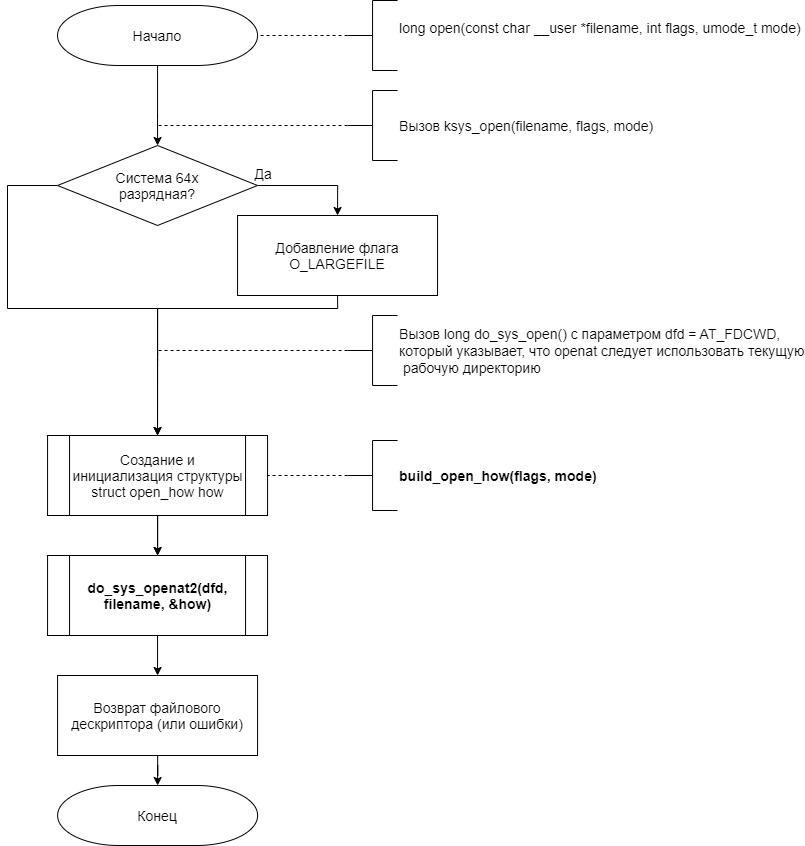
\includegraphics[scale=0.6]{img/open.jpg}
\end{figure}




\clearpage
\section{build\_open\_how()}

\begin{lstlisting}[language=c, caption=Структура open\_how и функция build\_open\_how()]
/*
Arguments for how openat2(2) should open the target path. If only @flags and @mode are non-zero, then openat2(2) operates very similarly to openat(2).
However, unlike openat(2), unknown or invalid bits in @flags result in -EINVAL rather than being silently ignored. @mode must be zero unless one of {O_CREAT, O_TMPFILE} are set.

 * @flags: O_* flags.
 * @mode: O_CREAT/O_TMPFILE file mode.
 * @resolve: RESOLVE_* flags.
 */
 
struct open_how {
	__u64 flags;
	__u64 mode;
	__u64 resolve;
};

/* List of all valid flags for the open/openat flags argument: */
#define VALID_OPEN_FLAGS \
	(O_RDONLY | O_WRONLY | O_RDWR | O_CREAT | O_EXCL | O_NOCTTY | O_TRUNC | \
	 O_APPEND | O_NDELAY | O_NONBLOCK | __O_SYNC | O_DSYNC | \
	 FASYNC	| O_DIRECT | O_LARGEFILE | O_DIRECTORY | O_NOFOLLOW | O_NOATIME | O_CLOEXEC | O_PATH | __O_TMPFILE)
	 
#define S_IALLUGO	(S_ISUID|S_ISGID|S_ISVTX|S_IRWXUGO)
#define WILL_CREATE(flags)	(flags & (O_CREAT | __O_TMPFILE))
#define O_PATH_FLAGS		(O_DIRECTORY | O_NOFOLLOW | O_PATH | O_CLOEXEC)

inline struct open_how build_open_how(int flags, umode_t mode)
{
	struct open_how how = {
		.flags = flags & VALID_OPEN_FLAGS,
		.mode = mode & S_IALLUGO,};
	/* O_PATH beats everything else. */
	if (how.flags & O_PATH)
		how.flags &= O_PATH_FLAGS;
	/* Modes should only be set for create-like flags. */
	if (!WILL_CREATE(how.flags))
		how.mode = 0;
	return how;
}
\end{lstlisting}


\begin{figure}[H]
	\centering
	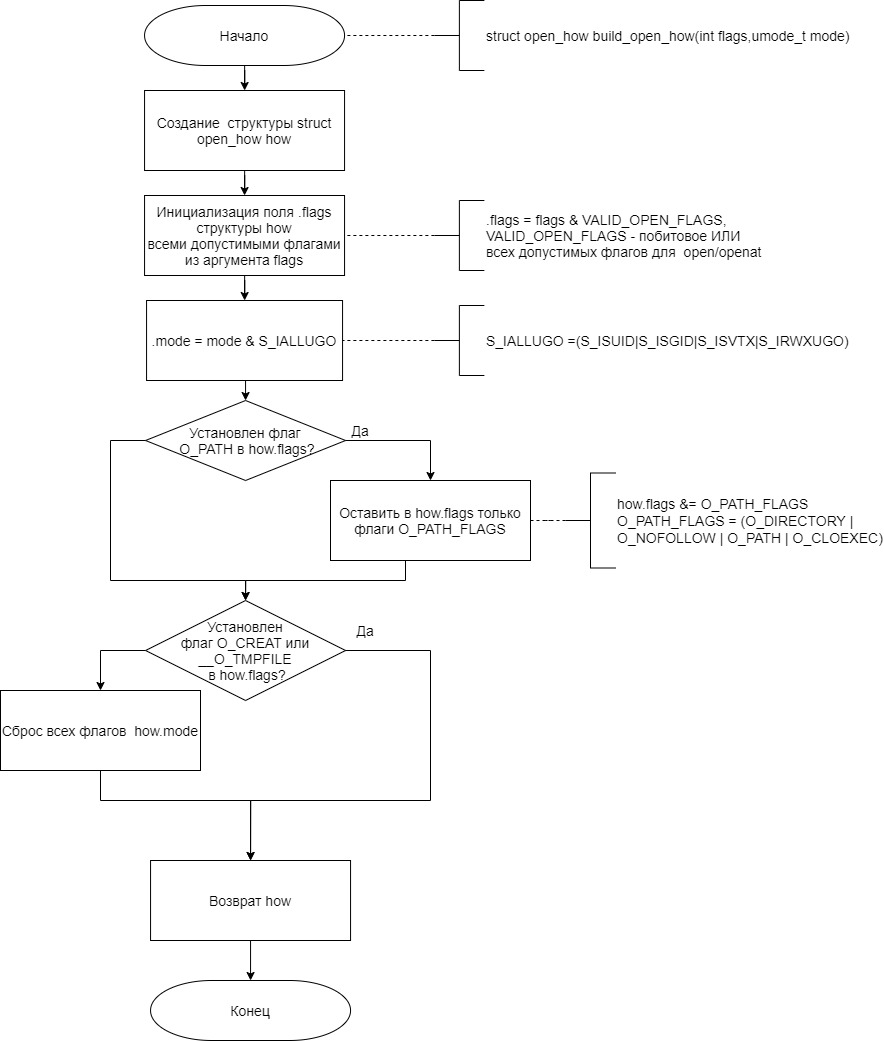
\includegraphics[scale=0.5]{img/build_open_how.jpg}
\end{figure}








\section{do\_sys\_openat2()}
\begin{figure}[H]
	\centering
	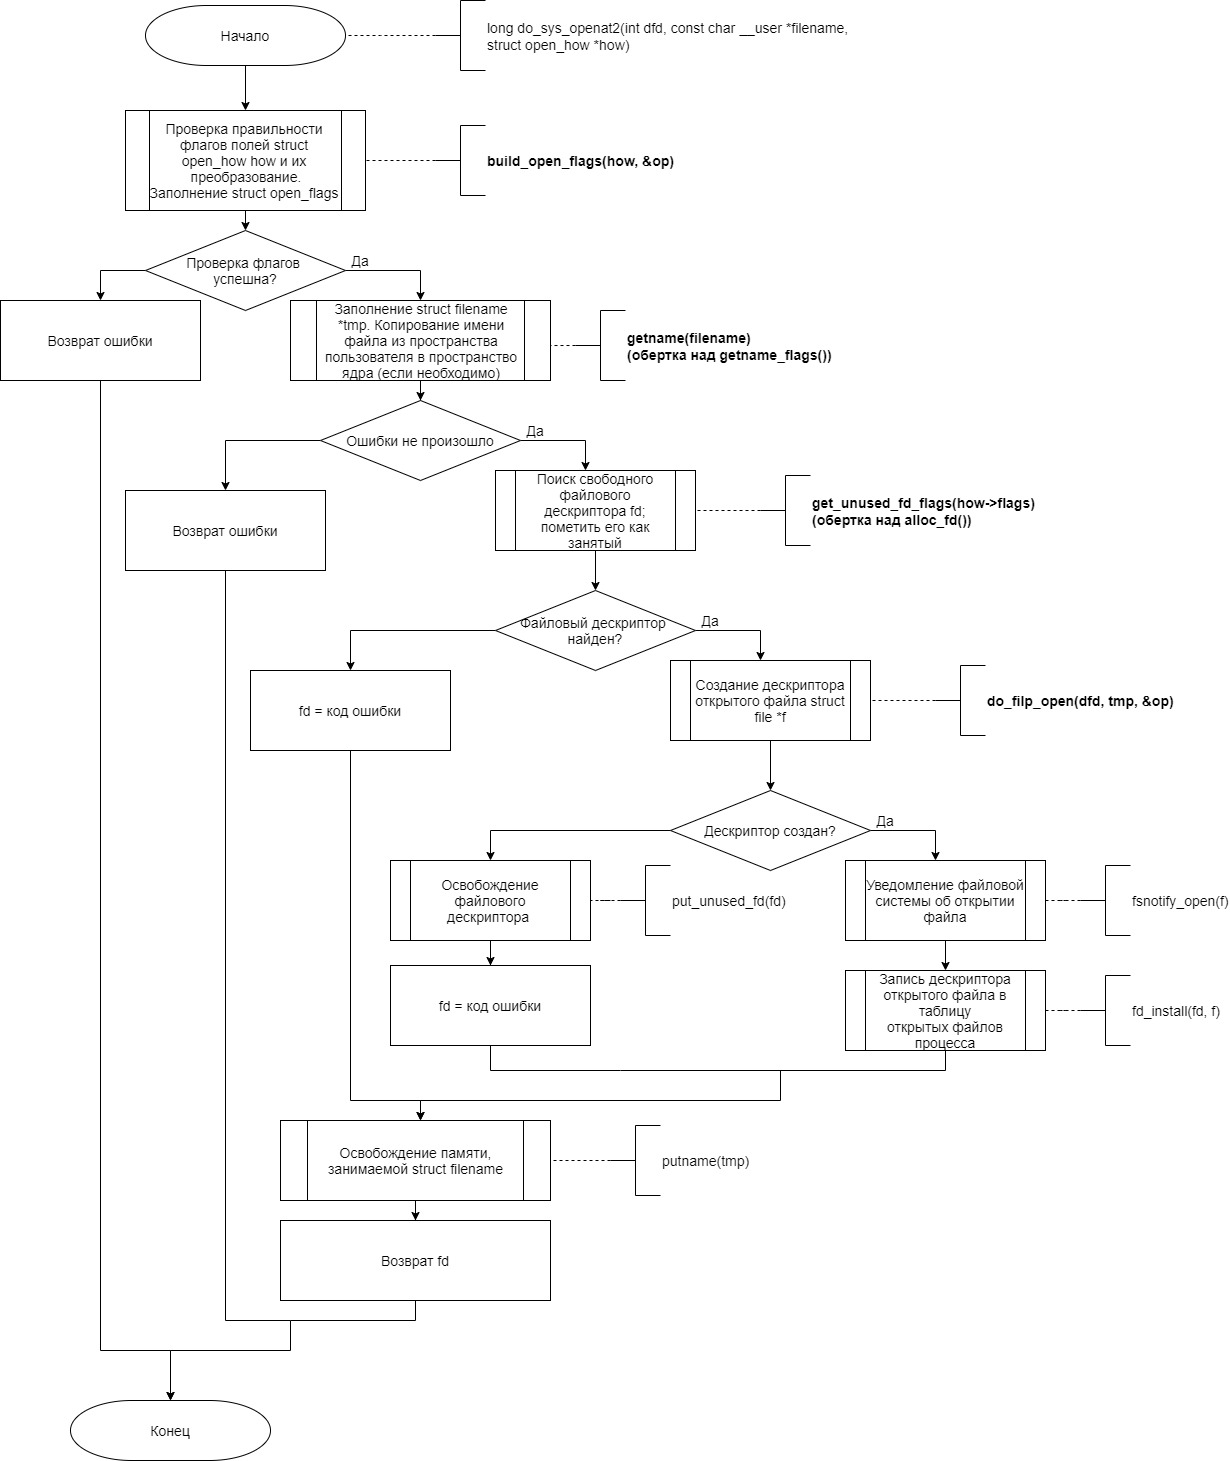
\includegraphics[scale=0.4]{img/do_sys_openat2.jpg}
\end{figure}



\clearpage
\section{build\_open\_flags()}

\begin{lstlisting}[language=c, caption=Структура open\_flags]
	
	struct open_flags {
		int open_flag;
		umode_t mode;
		int acc_mode;
		int intent;
		int lookup_flags;
	};
\end{lstlisting}

\begin{figure}[H]
	\centering
	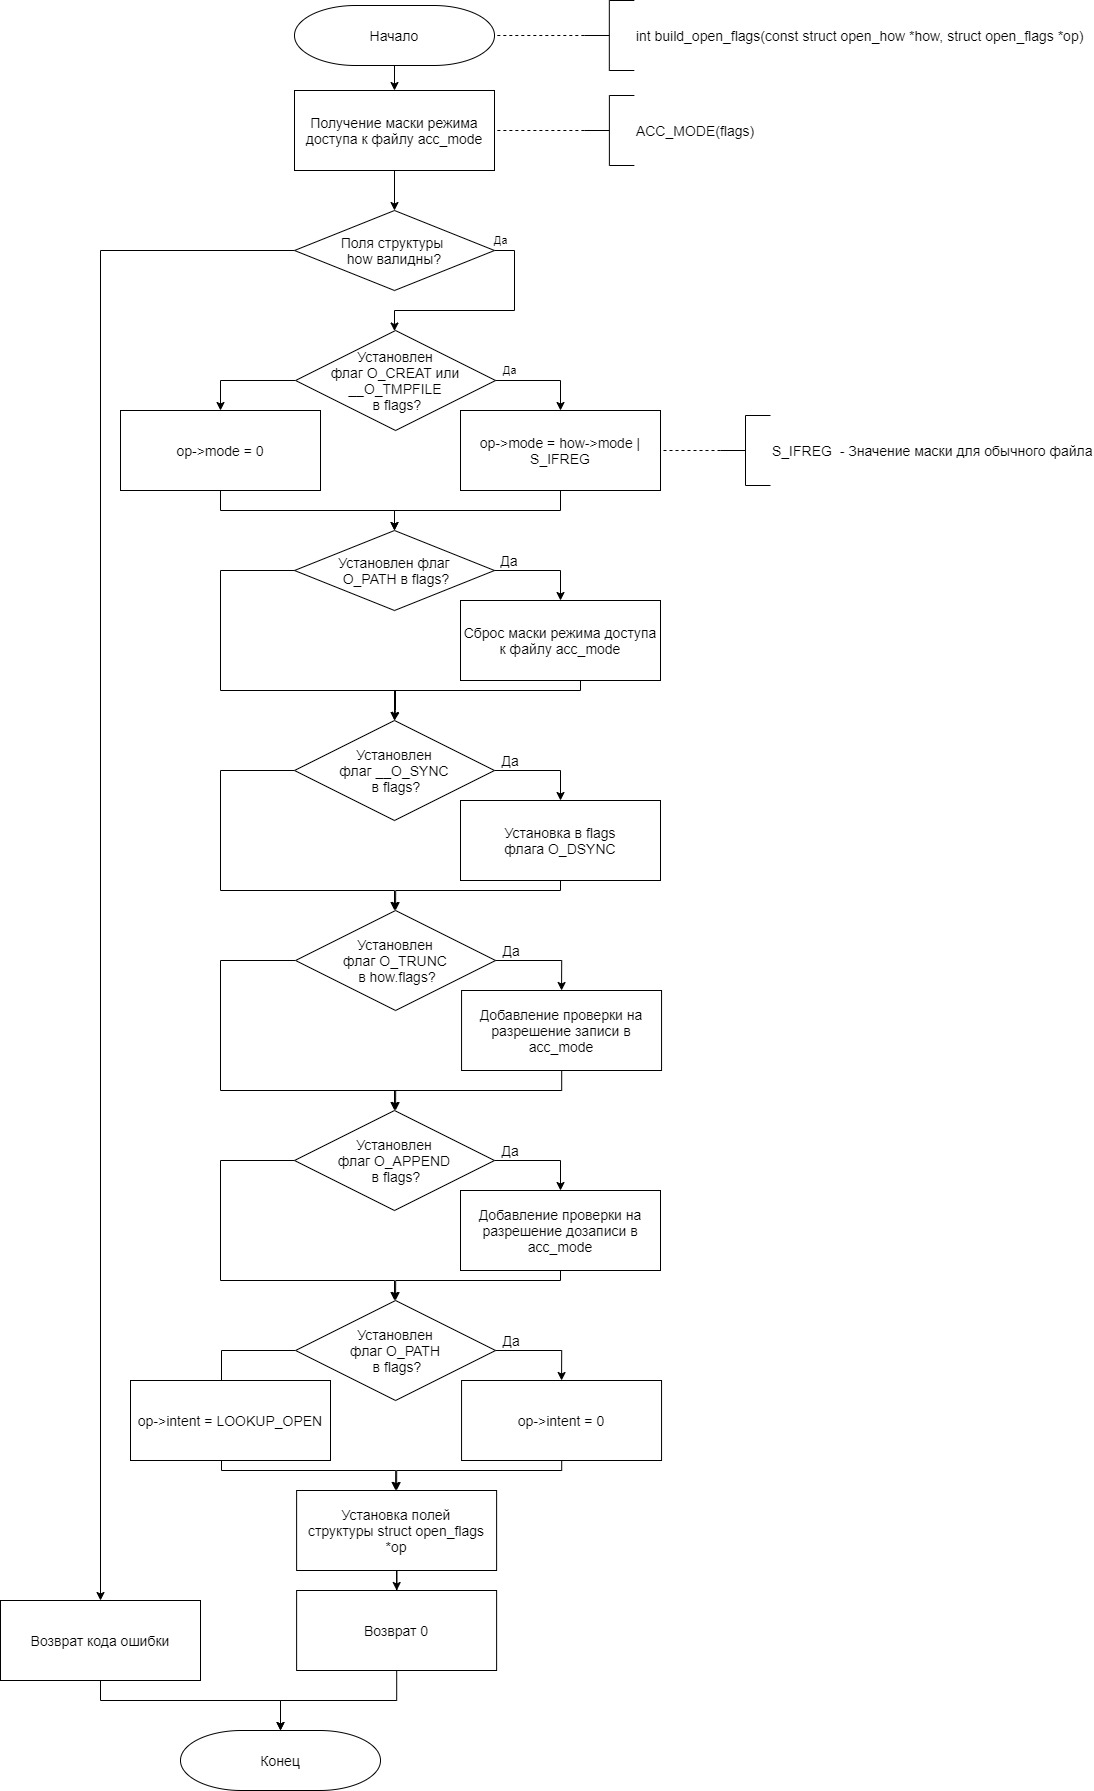
\includegraphics[scale=0.4]{img/build_open_flags.jpg}
\end{figure}





















\section{getname\_flags()}

\begin{lstlisting}[language=c, caption=Структуры audit\_names и filename]
struct audit_names;

struct filename {
	const char		*name;	/* pointer to actual string */
	const __user char	*uptr;	/* original userland pointer */
	int			refcnt;
	struct audit_names	*aname;
	const char		iname[];
};

struct audit_names {
	struct list_head	list;	/* audit_context->names_list */
	
	struct filename		*name;
	int			name_len;	/* number of chars to log */
	bool			hidden;	/* don't log this record */
	
	unsigned long		ino;
	dev_t			dev;
	umode_t			mode;
	kuid_t			uid;
	kgid_t			gid;
	dev_t			rdev;
	u32			osid;
	struct audit_cap_data	fcap;
	unsigned int		fcap_ver;
	unsigned char		type;		/* record type */
	/*
	* This was an allocated audit_names and not from the array of names allocated in the task audit context.  * Thus this name should be freed on syscall exit.
	*/
	bool			should_free;
};

\end{lstlisting}


%Когда вызывается getname(), указатель сохраняется в name и инкрементируется refcnt в ассоциированной struct filename.

%Далее, в  path\_lookup () сохраняется inode и device.



\begin{figure}[H]
	\centering
	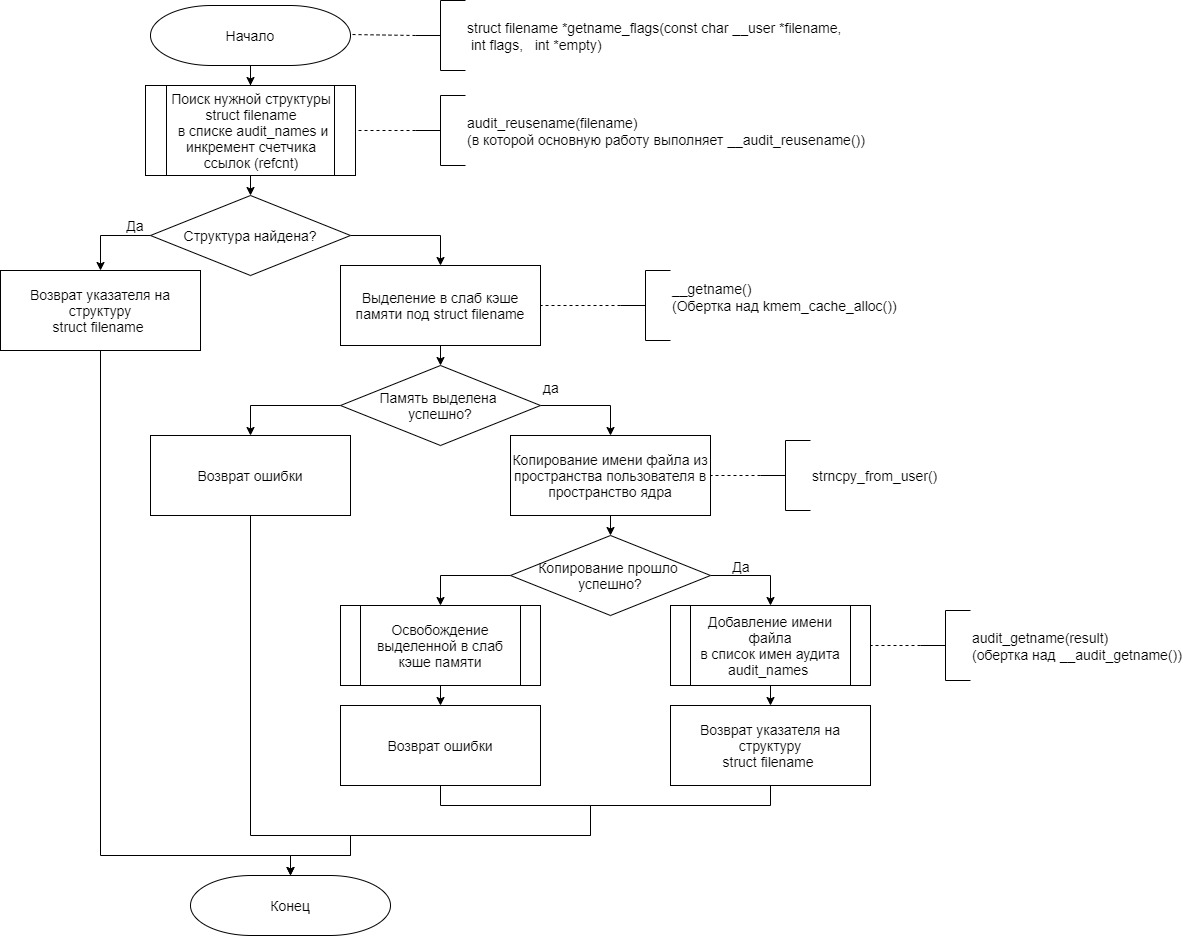
\includegraphics[scale=0.42]{img/getname_flags.jpg}
\end{figure}






\section{alloc\_fd}

\begin{figure}[H]
	\centering
	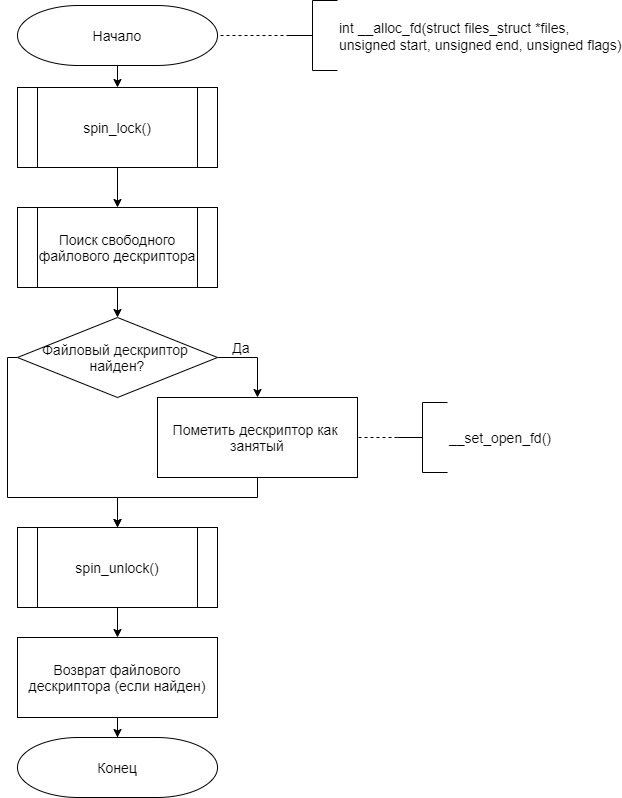
\includegraphics[scale=0.6]{img/alloc_fd.jpg}
\end{figure}







\section{do\_filp\_open}

\begin{figure}[H]
	\centering
	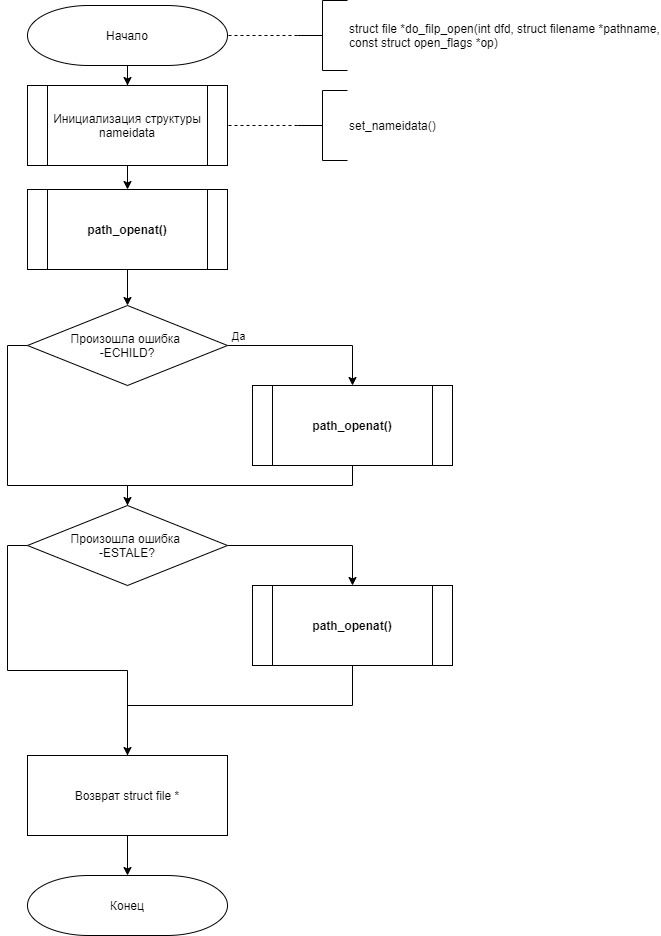
\includegraphics[scale=0.45]{img/do_filp_open.jpg}
	%\caption{Схема структур программы №1}
	\label{fig:do_filp_open}
\end{figure}







\section{set\_nameidata() и resotre\_nameidata()}

\begin{lstlisting}[language=c, caption=Структура nameidata]
struct nameidata {
	struct path	path;
	struct qstr	last;
	struct path	root;
	struct inode	*inode; /* path.dentry.d_inode */
	unsigned int	flags, state;
	unsigned	seq, m_seq, r_seq;
	int		last_type;
	unsigned	depth;
	int		total_link_count;
	struct saved {
		struct path link;
		struct delayed_call done;
		const char *name;
		unsigned seq;
	} *stack, internal[EMBEDDED_LEVELS];
	struct filename	*name;
	struct nameidata *saved;
	unsigned	root_seq;
	int		dfd;
	kuid_t		dir_uid;
	umode_t		dir_mode;
} __randomize_layout;

\end{lstlisting}

\begin{figure}[H]
	\centering
	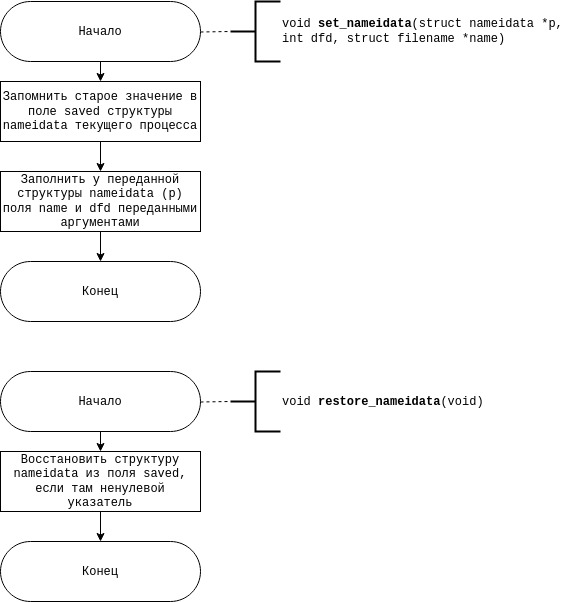
\includegraphics[scale=0.55]{img/nameidata.jpg}
\end{figure}




\section{path\_openat}

\begin{figure}[H]
	\centering
	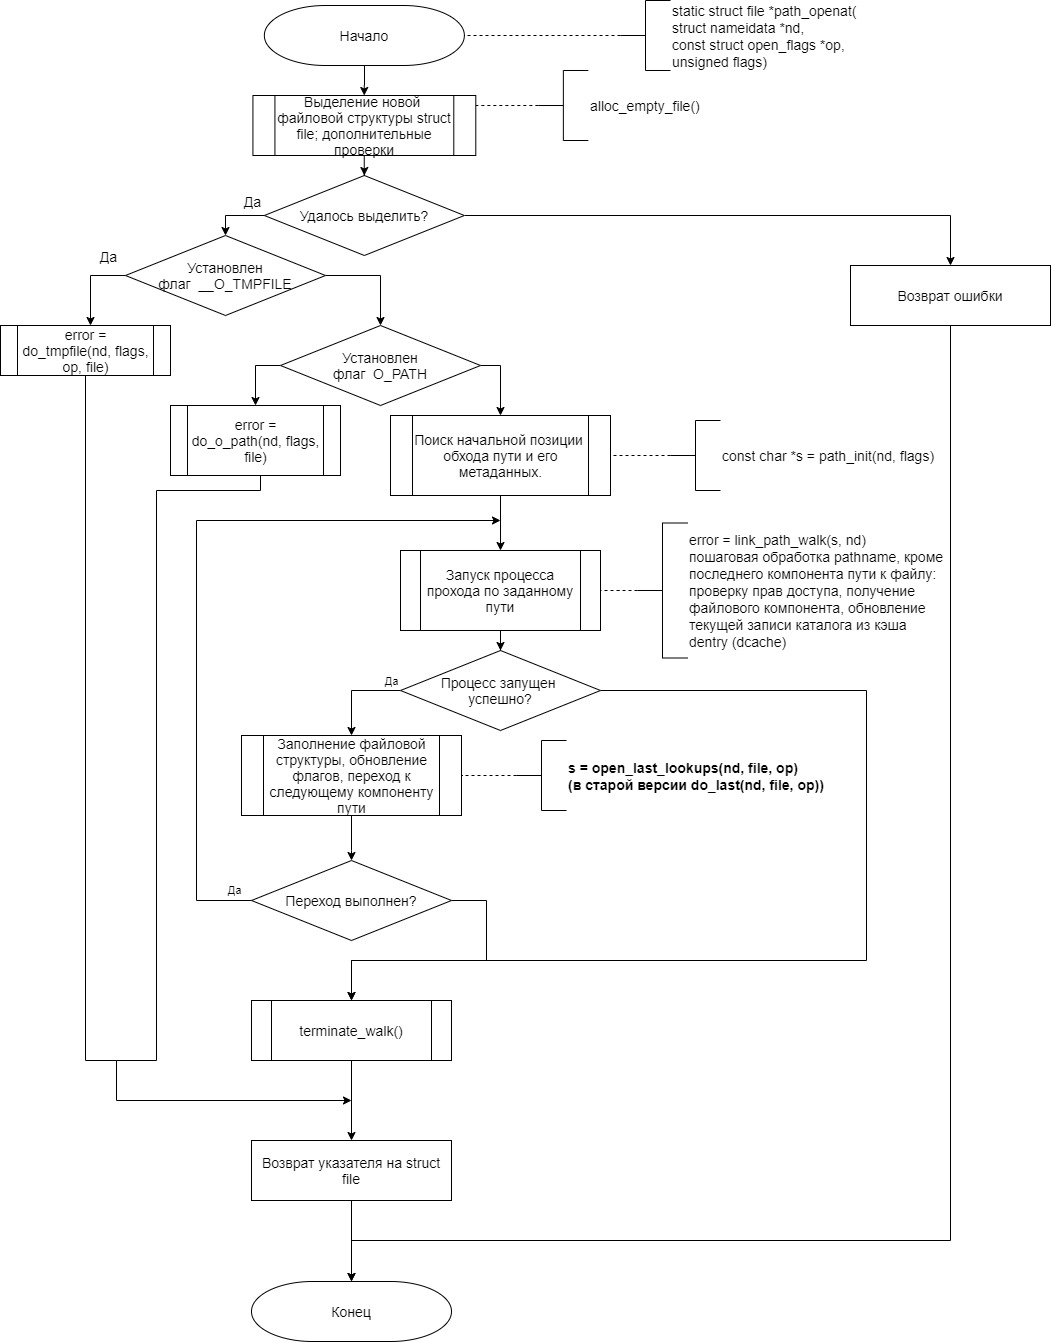
\includegraphics[scale=0.45]{img/path_openat.jpg}
\end{figure}








\section{open\_last\_lookups}

\begin{figure}[H]
	\centering
	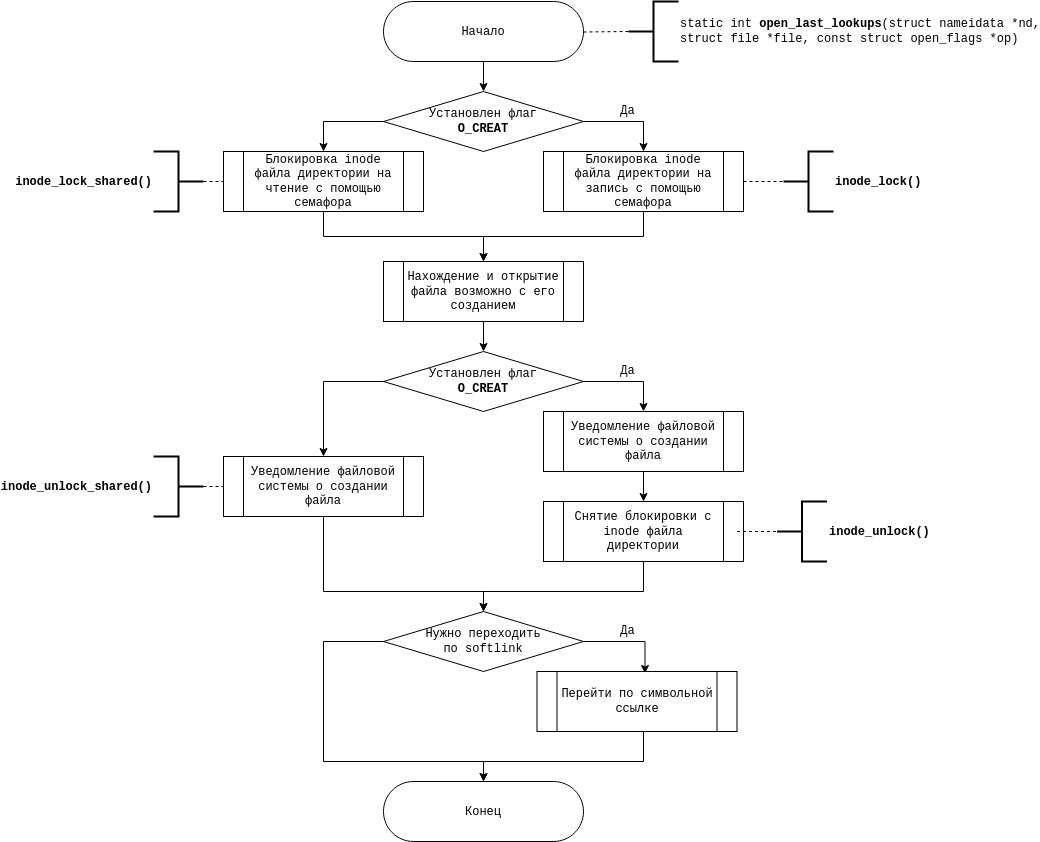
\includegraphics[scale=0.45]{img/open_last_lookups.jpg}
\end{figure}













\section{lookup\_open}

\begin{figure}[H]
	\centering
	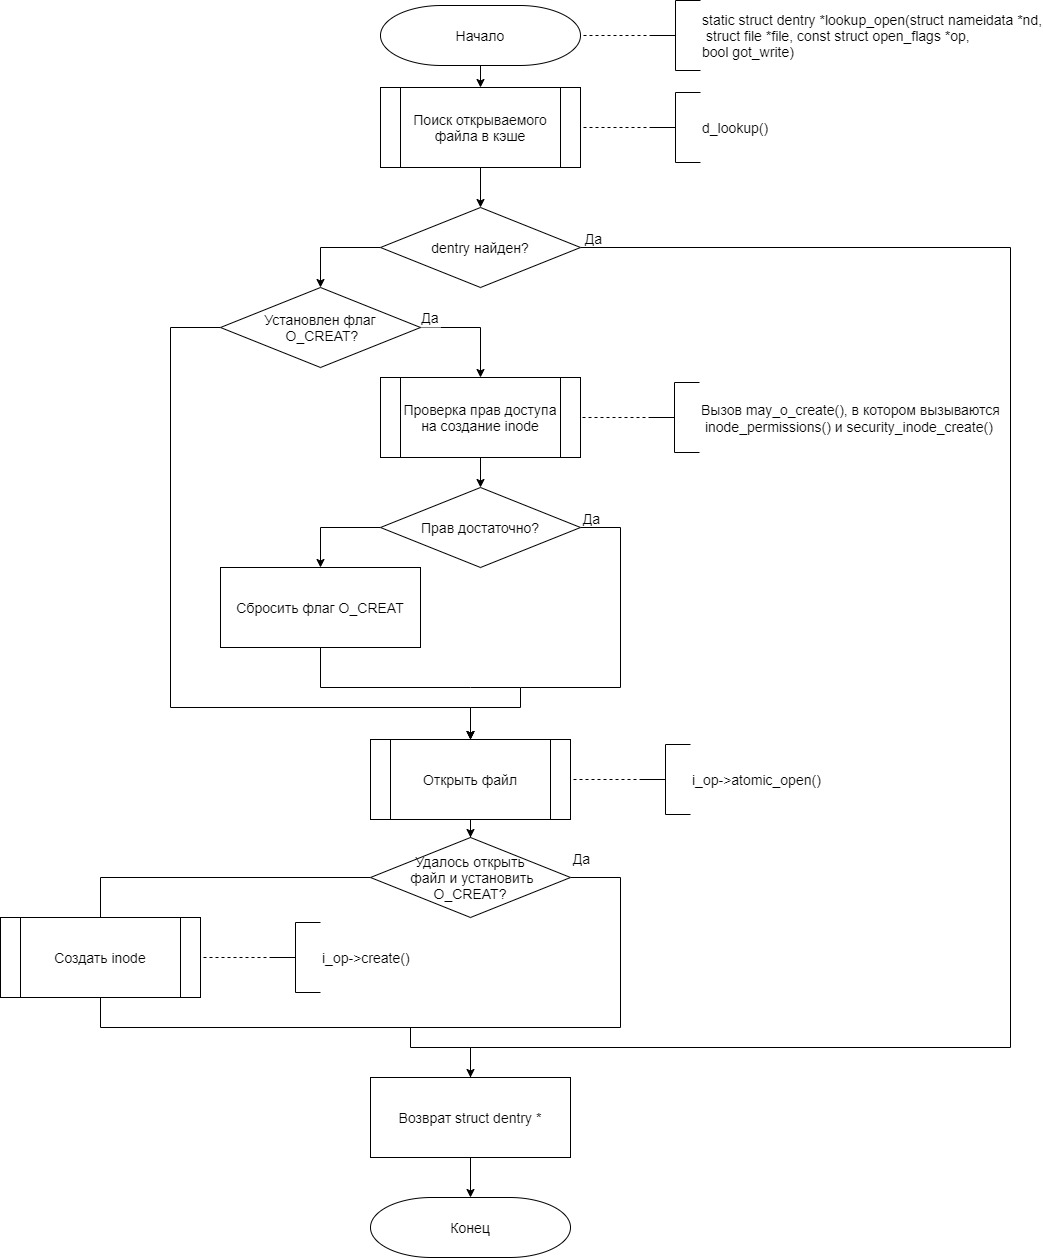
\includegraphics[scale=0.45]{img/lookup_open.jpg}
\end{figure}





















\bibliographystyle{utf8gost705u}  % стилевой файл для оформления по ГОСТу
\bibliography{51-biblio}          % имя библиографической базы (bib-файла)
	
\end{document}
